\subsection{Felügyelt és felügyelet nélküli tanulás. Mesterséges neurális hálózatok.}

\textbf{Neurális hálózatok:}
\begin{itemize}
    \item agyi neuronok működését leutánzó számítási egységek
    \item minták formájában reprezentált tudás megtanulására képes
    \item tudás típusai:
    \begin{itemize}
        \item analitikus, pl. matematikai egyenletek
        \item szabályalapú, pl. fuzzy rendszerek
        \item tapasztalati: minták, megfigyelések
    \end{itemize}
    \item neuronok biológiában:
    \begin{itemize}
        \item feladat: jelek vétele, kombinálása
        \item ha a kombinált jel elég erős, a neuron tüzel: kimenet
    \end{itemize}
    \item tanulás – programozás:
    \begin{center}
        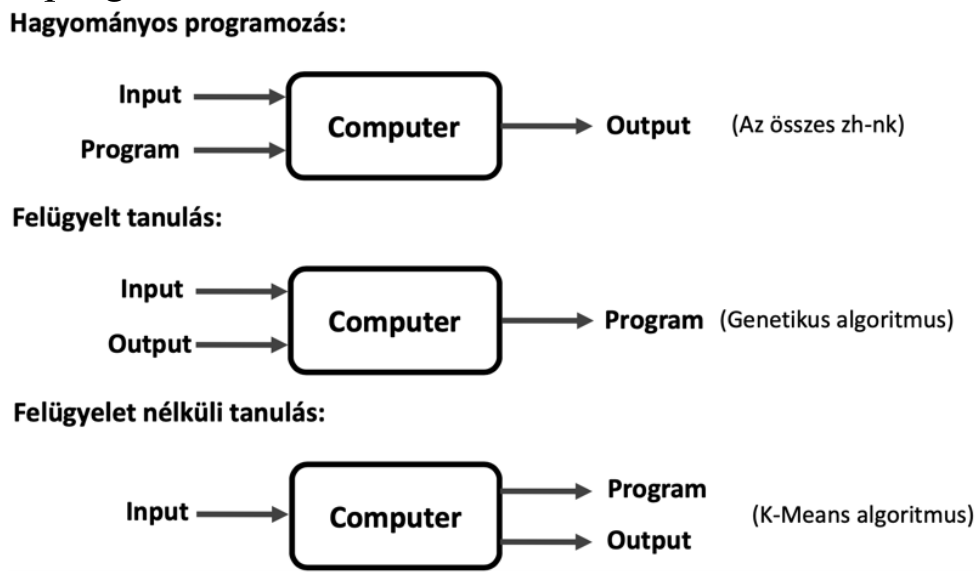
\includegraphics[width=0.6\textwidth]{res/imgs/info_26_learning_types.png}
    \end{center}
    \item mesterséges neuron:
    \begin{center}
        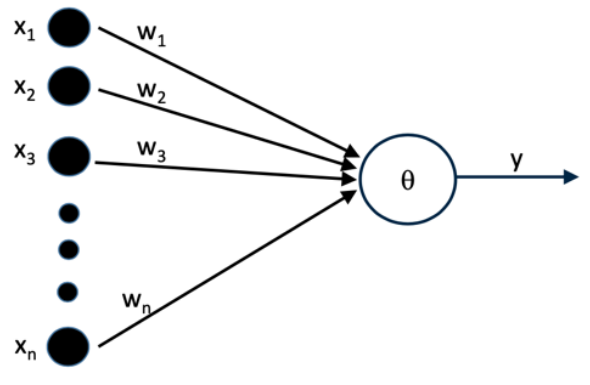
\includegraphics[width=0.4\textwidth]{res/imgs/info_26_artificial_neuron.png}
    \end{center}
    \begin{itemize}
        \item bemenetek: bejövő jelek $x_i$
        \item kimenet: klaszifikáció $y$
        \item súlyok: $w_i$
        \item küszöb: $\Theta$
        \item csak néhány egyszerű információ feldolgozására képes
        \item nem képes összetett problémák megoldására
        \item neuronok összekötve képesek komplex viselkedésre, így használhatók komplex problémák megoldására
    \end{itemize}
    \item felügyelt tanulás: \\
    adott: input-output tanító minták ($x_1^{(p)}, x_2^{(p)}, \dots, x_n^{(p)}, t^{(p)}$) \\
    $p$ darab minta, $n$ dimenziós input, skalár output
    \begin{center}
        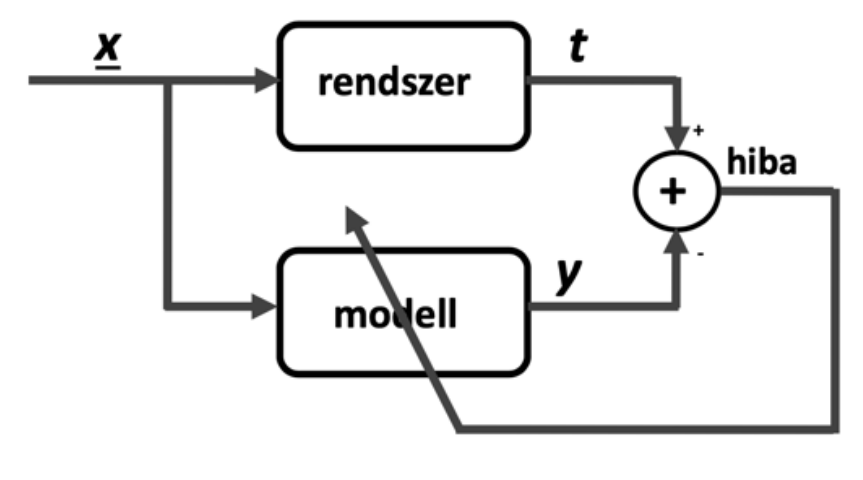
\includegraphics[width=0.4\textwidth]{res/imgs/info_26_supervised_learning_system.png}
    \end{center}
\end{itemize}

\textbf{Mesterséges neurális hálózatok (ANN):}
\begin{itemize}
    \item adat feldolgozó rendszerek
    \item nagy számú egyszerű, összekapcsolt feldolgozó elemek (mesterséges neuronok) architektúrája
    \item az agy komplex viselkedésre képes szerkezete inspirálta
    \item a neuronok rétegek sorozatába vannak rendezve
    \begin{itemize}
        \item teljes vagy részleges kapcsolat a rétegek közt
    \end{itemize}
    \item ugyanabban a rétegben elhelyezkedő neuronok aktivációs függvénye megegyezik
    \item a neurális hálózatok bemenetét a rendelkezésre álló adatok és az adatok előkészítése határozza meg
    \item kimenetét a célfeladat határozza meg
    \item rejtett rétegének mélységét a döntési összetettsége határozza meg
    \item szélességét a döntéshez szükséges adatok mennyisége határozza meg
    \item a hálózat megfelelő méretei általában nem előre meghatározhatók
    \item teljesen kapcsolt mesterséges neurális hálózatok
    \begin{itemize}
        \item egy adott réteg összes neuronja kapcsolatban áll a következő réteg összes neuronjával
        \item előny: egyszerű felépítés, maximális kihasználtság
        \item hátrány: sok memóriát igényel, sok számítást igényel
    \end{itemize}
    \begin{center}
        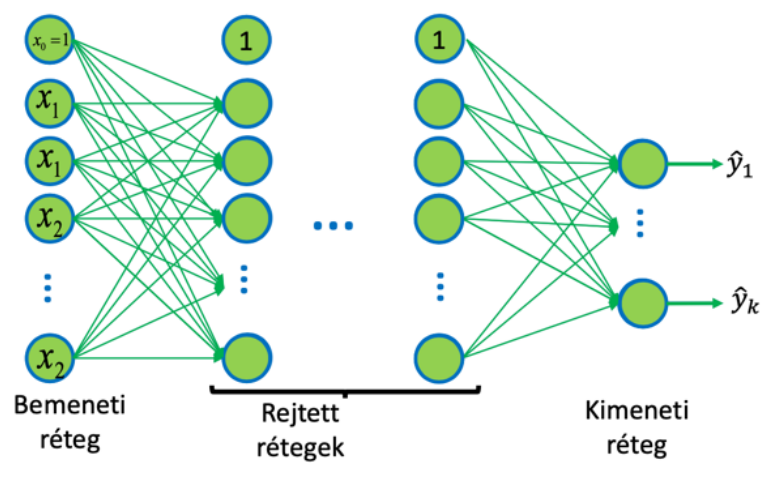
\includegraphics[width=0.7\textwidth]{res/imgs/info_26_fully_connected_ann.png}
    \end{center}
    \item részlegesen kapcsolt mesterséges neurális hálózatok
    \begin{itemize}
        \item egy adott réteg összes neuronja a következő rétegből csak néhány neuronnal áll kapcsolatban
    \end{itemize}
    \item csoportosítás jelfolyam szerint
    \begin{itemize}
        \item \begin{minipage}[t]{0.65\textwidth} előrecsatolt \end{minipage} \begin{minipage}[t]{0.3\textwidth} \vspace{-15pt} \begin{flushright} 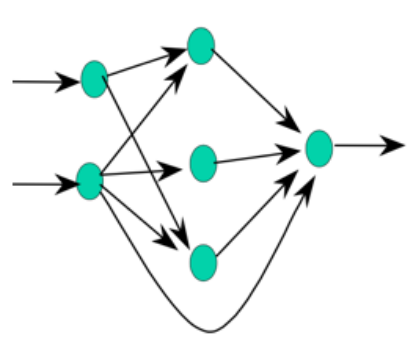
\includegraphics[width=\textwidth]{res/imgs/info_26_feedforward_ann.png} \end{flushright} \end{minipage}
        \begin{itemize}
            \item időben független adatok gyors feldolgozása
            \item időben függő adatok nem valós idejű pontos feldolgozása
        \end{itemize}
        \item \begin{minipage}[t]{0.75\textwidth} celluláris \end{minipage} \begin{minipage}[t]{0.2\textwidth} \vspace{-15pt} \begin{flushright} 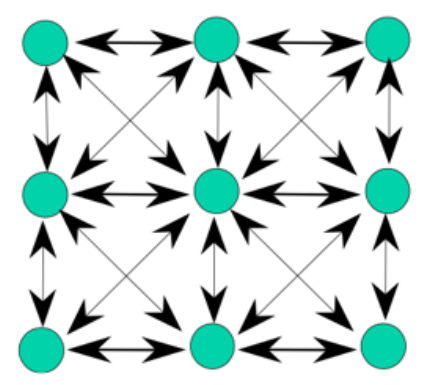
\includegraphics[width=\textwidth]{res/imgs/info_26_cellular_ann.png} \end{flushright} \end{minipage}
        \begin{itemize}
            \item csak a szomszédos egységek között van kapcsolat
            \item főleg képfeldolgozásra
        \end{itemize}
        \item \begin{minipage}[t]{0.65\textwidth} visszacsatolt \end{minipage} \begin{minipage}[t]{0.3\textwidth} \vspace{-15pt} \begin{flushright} 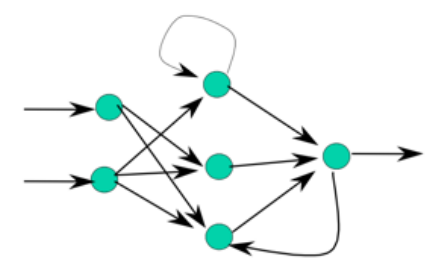
\includegraphics[width=\textwidth]{res/imgs/info_26_recurrent_ann.png} \end{flushright} \end{minipage}
        \begin{itemize}
            \item időben függő adatok gyors feldolgozása
        \end{itemize}
    \end{itemize}
\end{itemize}